% ============================
% TP Report – Simple Two-Column Template
% ============================
\documentclass[10pt,a4paper,twocolumn]{article}

% ---- Encoding & typography (simple, portable) ----
\usepackage[utf8]{inputenc}
\usepackage[T1]{fontenc}
\usepackage{lmodern}
\usepackage{microtype}

% ---- Layout ----
\usepackage{geometry}
\geometry{
  left=1.5cm, right=1.5cm,
  top=1.6cm, bottom=1.6cm,
  columnsep=0.6cm
}
\usepackage{balance} % balances the final page columns

% ---- Graphics ----
\usepackage{graphicx}
\usepackage[font=small,labelfont=bf]{caption}

% ---- Useful tweaks (optional) ----
\setlength{\parskip}{0pt}   % compact paragraphs
\setlength{\parindent}{1em} % classic indent; comment out if you prefer no indents

% ============================
%            Title
% ============================
\title{\vspace{-6mm}\textbf{TP Report Title: Short and Informative}}
\author{BONDIL Maxime - DE BACKER Mathis - DURAND Nicolas \quad G1 Polytech \\ Instructor: Mahdi Khoramshahi }
\date{\today}

\begin{document}
\maketitle

% ============================
%         One-sentence intro
% ============================
% Keep this to 2–3 lines max; no abstract section to stay minimal.
\noindent\textbf{Context.}
Dans ce TP nous avons tester des situations où l'on peut découplé les équations et annuler certaines inconnues des équations nous permettant d'isoler et d'identifier un plus petit groupe d'inconnues, pour ensuite identifier les plus complexes. 


% ============================
%           Sections
% ============================
\section*{Problem Statement}
Les inconnues des équations du système comprennent les termes d’inertie, centrifuges, de gravité et de frottements. De plus, les deux équations du système sont couplées dans un sens, car le mouvement du premier moteur engendre une rotation du deuxième.
On cherche ensuite à traiter chaque moteur séparément. On établit des situations où les deux moteurs sont découplés, ce qui nous donne : les termes d’inertie et centrifuges sont nuls, et les termes de gravité sont découplés, pour ainsi pouvoir identifier les paramètres gravitaires et de frottements restants.
Grâce aux paramètres trouvés, on peut maintenant isoler et déterminer les paramètres manquants d’inertie et ceux centrifuges.

\section*{Method and Implementation}
On a fait attention à ce que le nombre "n" de données (q1, q2, qp1, qp2 ...) soit bien dimensionné en fonctions des paramètres que l'on étudie en utilisant : n = size(q1).
Comme pour le TP1 on a fait deux matrices (A et u) qui s'ajustent en fonction du nombre de données.
En utilisant la formule du cours on peut verifie que les parametres trouvés on la même échelle d'erreur.

% ============================
%     Main Results Figure
% ============================
% Use figure* to span both columns. Replace results.pdf with your image file.
\begin{figure}[!h]
  \centering
  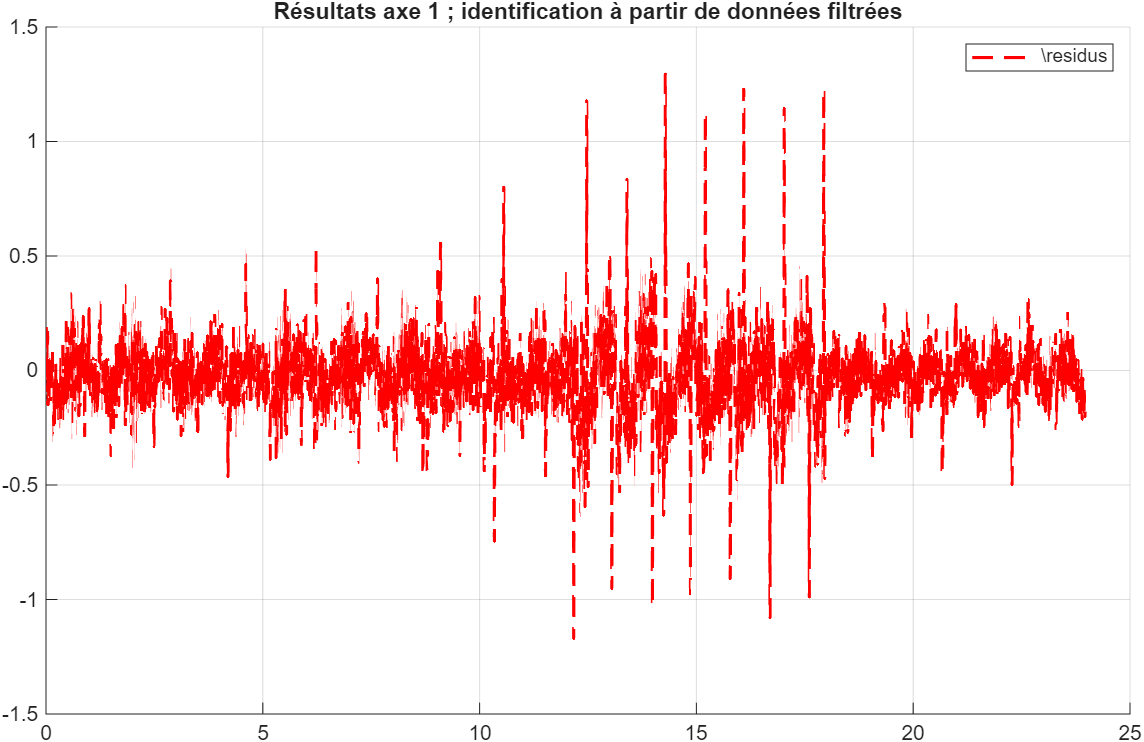
\includegraphics[width=0.45\textwidth]{fig_parameters.png}
  \caption{Résultats axe 1 ; identification à partir de données filtrées}
  \label{fig:summary}
\end{figure}

\section*{Results}
On observe que les paramètres filtrés nous donnent des valeurs assez proches (ou identiques) par rapport à ceux non filtrés, mais on ne sait pas les plus véridicte, même si l'on suppose que ceux filtrés sont plus exacts.\\
On observe sur le graphique \ref{fig:summary} que la différence entre le signal de sortie trouvé et le signal réel ressemble a une sinusoïde très bruitée qui correspond à l'élément que l'on n'a pas pris en compte lors de notre étude : la courroie.

\section*{Conclusion}
On a aprris qu'il fallait découpler notre système pour pouvoir en identifier les paramètres, et ne pas hésiter à annuler le plus de termes possible avant de les rajouter au fur et à mesure. Il ne faut pas oublier que ce que l'on ne modelise pas (comme la courroie) par simplicité a toujours une répercussion sur le résultat final.

% Balance last page columns and end.
\balance

\end{document}
